\documentclass[a4paper]{article}
    \usepackage[pdftex]{hyperref}
    \usepackage[latin1]{inputenc}
    \usepackage[english]{babel}
    \usepackage{a4wide}
    \usepackage{amsmath}
    \usepackage{amssymb}
    \usepackage{algorithmic}
    \usepackage{algorithm}
    \usepackage{ifthen}
    \usepackage{listings}
    % move the asterisk at the right position
    \lstset{basicstyle=\ttfamily,tabsize=4,literate={*}{${}^*{}$}1}
    %\lstset{language=C,basicstyle=\ttfamily}
    \usepackage{moreverb}
    \usepackage{palatino}
    \usepackage{multicol}
    \usepackage{tabularx}
    \usepackage{comment}
    \usepackage{verbatim}
    \usepackage{color}
    \usepackage{enumitem}
    \usepackage{tikz}
    \usetikzlibrary{arrows,shapes.gates.logic.US,shapes.gates.logic.IEC,calc}
    
    \usepackage[left=3cm, right=3cm, top=4cm, bottom=4cm]{geometry}
    
    \usepackage{graphicx}
    
    %% pdflatex?
    \newif\ifpdf
    \ifx\pdfoutput\undefined
    \pdffalse % we are not running PDFLaTeX
    \else
    \pdfoutput=1 % we are running PDFLaTeX
    \pdftrue
    \fi
    \ifpdf
    \usepackage[pdftex]{graphicx}
    \else
    \usepackage{graphicx}
    \fi
    \ifpdf
    \DeclareGraphicsExtensions{.pdf, .jpg}
    \else
    \DeclareGraphicsExtensions{.eps, .jpg}
    \fi
    
    \parindent=0cm
    \parskip=0cm
    
    \setlength{\columnseprule}{0.4pt}
    \addtolength{\columnsep}{2pt}
    
    \addtolength{\textheight}{5.5cm}
    \addtolength{\topmargin}{-26mm}
    \pagestyle{empty}
    
    %%
    %% Sheet setup
    %% 
    \newcommand{\coursename}{Computer Architecture and Programming Languages}
    \newcommand{\courseno}{CO20-320241}
     
    \newcommand{\sheettitle}{Homework}
    \newcommand{\mytitle}{}
    \newcommand{\mytoday}{\textcolor{blue}{September 25}, 2018}
    
    % Current Assignment number
    \newcounter{assignmentno}
    \setcounter{assignmentno}{2}
    
    % Current Problem number, should always start at 1
    \newcounter{problemno}
    \setcounter{problemno}{1}
    
    %%
    %% problem and bonus environment
    %%
    \newcounter{probcalc}
    \newcommand{\problem}[2]{
      \pagebreak[2]
      \setcounter{probcalc}{#2}
      ~\\
      {\large \textbf{Problem \textcolor{blue}{\arabic{assignmentno}}.\textcolor{blue}{\arabic{problemno}}} \hspace{0.2cm}\textit{#1}} \refstepcounter{problemno}\vspace{2pt}\\}
    
    \newcommand{\bonus}[2]{
      \pagebreak[2]
      \setcounter{probcalc}{#2}
      ~\\
      {\large \textbf{Bonus Problem \textcolor{blue}{\arabic{assignmentno}}.\textcolor{blue}{\arabic{problemno}}} \hspace{0.2cm}\textit{#1}} \refstepcounter{problemno}\vspace{2pt}\\}
    
    %% some counters  
    \newcommand{\assignment}{\arabic{assignmentno}}
    
    %% solution  
    \newcommand{\solution}{\pagebreak[2]{\bf Solution:}\\}
    
    %% Hyperref Setup
    \hypersetup{pdftitle={Homework \assignment},
      pdfsubject={\coursename},
      pdfauthor={},
      pdfcreator={},
      pdfkeywords={Computer Architecture and Programming Languages},
      %  pdfpagemode={FullScreen},
      %colorlinks=true,
      %bookmarks=true,
      %hyperindex=true,
      bookmarksopen=false,
      bookmarksnumbered=true,
      breaklinks=true,
      %urlcolor=darkblue
      urlbordercolor={0 0 0.7}
    }
    
    \begin{document}
    \coursename \hfill Course: \courseno\\
    Jacobs University Bremen \hfill \mytoday\\
    \textcolor{blue}{Dushan Terzikj}\hfill
    \vspace*{0.3cm}\\
    \begin{center}
    {\Large \sheettitle{} \textcolor{blue}{\assignment}\\}
    \end{center}
    
    \problem{}{0}
    \solution
    \textcolor{blue}{
        \begin{enumerate}[label=(\alph*)]
            \item $777_8 + 1_8=1000_8$
            \item $888_{16} + 1_{16}=889_{16}$
            \item $32007_8 + 1_{8}=32010_{8}$
            \item $32108_{16} + 1_{16}=32109_{16}$
            \item $8BFF_{16} + 1_{16}=8C00_{16}$
            \item $1219_{16} + 1_{16} = 121A_{16}$
        \end{enumerate}
    }
    
    \problem{}{0}
    \solution
    \textcolor{blue}{
    \tikzstyle{branch}=[fill,shape=circle,minimum size=3pt,inner sep=0pt]
    \begin{enumerate}[label=(\alph*)]
        \item
        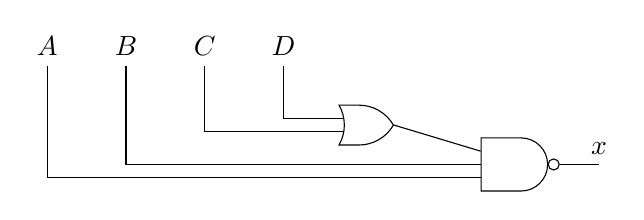
\begin{tikzpicture}[label distance=2mm]
            \node (A) at (0,0) {$ A $};
            \node (B) at (1,0) {$ B $};
            \node (C) at (2,0) {$ C $};
            \node (D) at (3,0) {$ D $};
            \node[or gate US, draw, logic gate inputs=nn] at ($(D)+(1,-1)$) (Or0) {};
            \node[nand gate US, draw, logic gate inputs=nnn] at ($(Or0.output)+(1.5,-0.5)$) (Nand0) {};
            \draw (C) |- (Or0.input 2);
            \draw (D) |- (Or0.input 1);
            \draw (A) |- (Nand0.input 3);
            \draw (B) |- (Nand0.input 2);
            \draw (Or0.output) -- (Nand0.input 1);
            \draw (Nand0.output) -- ([xshift=0.5cm]Nand0.output) node[above] {$ x $};
        \end{tikzpicture}
        \item
        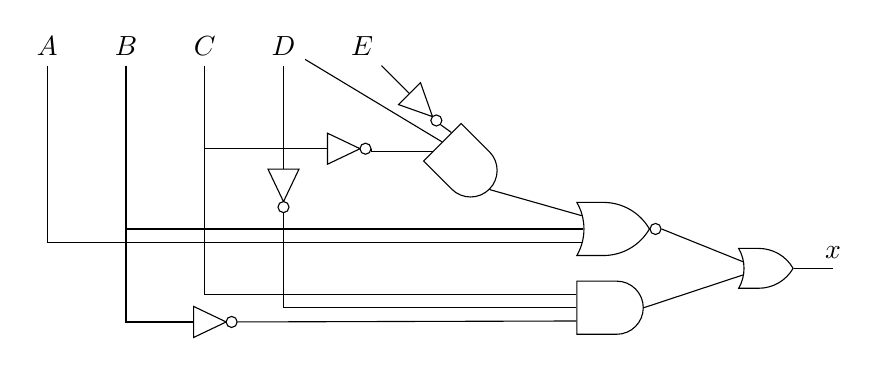
\begin{tikzpicture}[label distance=2mm]
            \node (A) at (0,0) {$ A $};
            \node (B) at (1,0) {$ B $};
            \node (C) at (2,0) {$ C $};
            \node (D) at (3,0) {$ D $};
            \node (E) at (4,0) {$ E $};
            \node[not gate US, draw] at ($(C)+(1.7,-1.3)$) (Not0) {};
            \node[not gate US, draw, rotate=-45] at ($(E)+(0.7,-0.7)$) (Not1) {};
            \node[not gate US, draw] at ($(C)+(0,-3.5)$) (Not2) {};
            \node[not gate US, draw, rotate=-90] at ($(D)+(0,-1.7)$) (Not3) {};
            \node[and gate US, draw, logic gate inputs=nnn, rotate=-45] at ($(Not1.output)+(0.3,-0.5)$) (And0) {};
            \node[nor gate US, draw, logic gate inputs=nnn] at ($(And0.output)+(1.5,-0.5)$) (Nor0) {};
            \node[and gate US, draw, logic gate inputs=nnn] at ($(Nor0)+(0,-1)$) (And1) {};
            \node[or gate US, draw, logic gate inputs=nn] at ($(And1.output)+(1.5,0.5)$) (Or0) {};
            \draw (C) |- (Not0.input);
            \draw (E) -- (Not1.input);
            \draw (Not1.output) -- (And0.input 1);
            \draw (D) -- (And0.input 2);
            \draw (Not0.output) |- (And0.input 3);
            \draw (Or0.output) -- ([xshift=0.5cm]Or0.output) node[above] {$ x $};
            \draw (And0.output) -- (Nor0.input 1);
            \draw (B) |- (Nor0.input 2);
            \draw (A) |- (Nor0.input 3);
            \draw (C) |- (And1.input 1);
            \draw (B) |- (Not2.input);
            \draw (Not2.output) -- (And1.input 3);
            \draw (D) -- (Not3.input);
            \draw (Not3.output) |- (And1.input 2);
            \draw (Nor0.output) -- (Or0.input 1);
            \draw (And1.output) -- (Or0.input 2);
        \end{tikzpicture}
        \item
        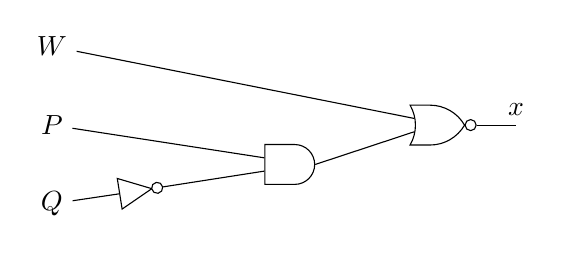
\begin{tikzpicture}[label distance=2mm]
            \node (W) at (0,0) {$ W $};
            \node (P) at (0,-1) {$ P $};
            \node (Q) at (0,-2) {$ Q $};
            \node[not gate US, draw, rotate=9] at ($(Q)+(1,0.15)$) (Not0) {};
            \node[and gate US, draw, logic gate inputs=nn] at ($(Q)+(3,0.5)$) (And0) {};
            \node[nor gate US, draw, logic gate inputs=nn] at ($(And0.output)+(1.5,0.5)$) (Nor0) {};
            \draw (Q) -- (Not0.input);
            \draw (Not0.output) -- (And0.input 2);
            \draw (P) -- (And0.input 1);
            \draw (W) -- (Nor0.input 1);
            \draw (And0.output) -- (Nor0.input 2);
            \draw (Nor0.output) -- ([xshift=0.5cm]Nor0.output) node[above] {$ x $};
        \end{tikzpicture}
        \item
        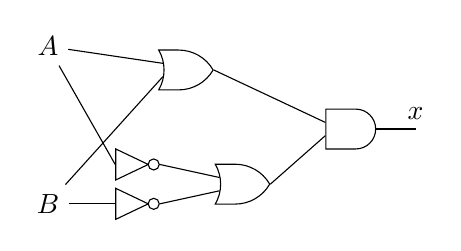
\begin{tikzpicture}[label distance=2mm]
            \node (A) at (0,0) {$ A $};
            \node (B) at (0,-2) {$ B $};
            \node[or gate US, draw, logic gate inputs=nn] at ($(A)+(1.7,-0.3)$) (Or0) {};
            \node[not gate US, draw] at ($(B)+(1,0.5)$) (Not0) {};
            \node[not gate US, draw] at ($(B)+(1,0)$) (Not1) {};
            \node[or gate US, draw, logic gate inputs=nn] at ($(Not1.output)+(1,0.25)$) (Or1) {};
            \node[and gate US, draw, logic gate inputs=nn] at ($(Or1.output)+(1,0.7)$) (And0) {};
            \draw (A) -- (Or0.input 1);
            \draw (B) -- (Or0.input 2);
            \draw (A) -- (Not0.input);
            \draw (B) -- (Not1.input);
            \draw (Not0.output) -- (Or1.input 1);
            \draw (Not1.output) -- (Or1.input 2);
            \draw (Or0.output) -- (And0.input 1);
            \draw (Or1.output) -- (And0.input 2);
            \draw (And0.output) -- ([xshift=0.5cm]And0.output) node[above] {$ x $};
        \end{tikzpicture}
    \end{enumerate}}
    
    
    \problem{}{0}
    \solution
    \textcolor{blue}{
        The algebraic expression for the logic circuit is the following:
        \begin{equation*}
            (\overline{\overline{(M\cdot N\cdot Q)}\cdot\overline{(M\cdot\overline{N}\cdot Q)}\cdot\overline{(\overline{M}\cdot N\cdot Q)}})
        \end{equation*}
        \\First let's denote $(\overline{\overline{(M\cdot N\cdot Q)}\cdot\overline{(M\cdot\overline{N}\cdot Q)}\cdot\overline{(\overline{M}\cdot N\cdot Q)}})=R$. The truth table for this expression is the following:\\ \\
        \begin{center}
            \begin{tabular}{|c|c|c|c|}
                \hline
                Q&N&M&R  \\
                \hline
                0&0&0&0  \\
                \hline
                0&0&1&0  \\
                \hline
                0&1&0&0  \\
                \hline
                0&1&1&0  \\
                \hline
                1&0&0&0  \\
                \hline
                1&0&1&1  \\
                \hline
                1&1&0&1  \\
                \hline
                1&1&1&1  \\
                \hline
            \end{tabular}
        \end{center}\\ \\
        Given the truth table of the circuit, we can obtain the sum of products (a.k.a, DNF, Disjunctive Normal Form) by writing down the product (conjunction) of the input values for every row where the result is 1 and connecting all obtained products (conjunctions) together with sum (disjunction) (references for this are the slides from Introduction to Computer Science from Choice Module General Computer Science which is held in Fall Semester at Jacobs University). Those rows are the last 3 rows in the truth table above. Therefore:
        \begin{equation}
            (Q\cdot \overline{N}\cdot M)+(Q\cdot N\cdot \overline{M})+(Q\cdot N\cdot M)
        \end{equation}
        We can simplify (1) by using the distributive rule, but it is not going to change much.
    }
    
    \problem{}{0}
    \solution
    \textcolor{blue}{
        \begin{enumerate}[label=(\alph*)]
            \item \begin{tabular}{|c|c|c|c|c|c|c|} \hline
                 X  &  Y  & $ \overline{\rm X} $ & $ \overline{\rm Y} $ & $ \overline{\rm X} \cdot Y $ & $ X + \overline{\rm X} \cdot Y $ & $ X + Y $ \\ 
                 \hline
                0 & 0 & 1 & 1 & 0 & 0 & 0 \\
                \hline
                0 & 1 & 1 & 0 & 1 & 1 & 1 \\
                \hline
                1 & 0 & 0 & 1 & 0 & 1 & 1 \\
                \hline
                1 & 1 & 0 & 0 & 0 & 1 & 1 \\ 
                \hline
                \end{tabular}
            \item \begin{tabular}{|c|c|c|c|c|c|c|} \hline
                 X  &  Y  & $ \overline{\rm X} $ & $ \overline{\rm Y} $ & $ X \cdot Y $ & $ \overline{\rm X} + X \cdot Y $ & $ \overline{\rm X} + Y $ \\ \hline
                0 & 0 & 1 & 1 & 0 & 1 & 1 \\
                \hline
                0 & 1 & 1 & 0 & 0 & 1 & 1 \\
                \hline
                1 & 0 & 0 & 1 & 0 & 0 & 0 \\
                \hline
                1 & 1 & 0 & 0 & 1 & 1 & 1 \\ 
                \hline
                \end{tabular}
        \end{enumerate}
    }
    
    \problem{}{0}
    \solution
    \textcolor{blue}{
        \begin{enumerate}[label=(\alph*)]
            \item $A+1=1$
            \item $A\cdot A=A$
            \item $B\cdot \overline{B}=0$
            \item $C+C=C$
            \item $x\cdot 0=0$
            \item $D\cdot 1=D$
            \item $D+0=D$
            \item $C+\overline{C}=1$
            \item $G+G\cdot F=G$
            \item $Y+\overline{W}\cdot Y=Y$
        \end{enumerate}
    }
    
    \newpage
    
    \problem{}{0}
    \solution
    \textcolor{blue}{
        First de Morgan's rule: $\overline{A+B}=\overline{A}\cdot \overline{B}$. Truth table:
        \begin{center}
            \begin{tabular}{|c|c|c|c|}
                \hline
                $A$&$B$&$\overline{A+B}$&$\overline{A}\cdot\overline{B}$  \\ \hline
                0&0&1&1  \\ \hline 
                0&1&0&0  \\ \hline 
                1&0&0&0  \\ \hline 
                1&1&0&0  \\ \hline 
            \end{tabular}
        \end{center}
        Second de Morgan's rule: $\overline{A\cdot B}=\overline{A}+\overline{B}$. Truth table:
        \begin{center}
            \begin{tabular}{|c|c|c|c|}
                \hline
                $A$&$B$&$\overline{A\cdot B}$&$\overline{A}+\overline{B}$  \\ \hline
                0&0&1&1  \\ \hline 
                0&1&1&1  \\ \hline 
                1&0&1&1  \\ \hline 
                1&1&0&0  \\ \hline 
            \end{tabular}
        \end{center}
    }
    
    \problem{}{0}
    \solution
    \textcolor{blue}{
        Given the truth table, we can obtain the sum of products by writing down the product of the input values for every row where the output results is 1 and connecting all obtained products together with addition (see problem 2.3 and its reference). Therefore we have:
        \begin{align}
            &\overline{A}\cdot\overline{B}\cdot\overline{C}\cdot D + \overline{A}\cdot\overline{B}\cdot C\cdot D + \overline{A}\cdot B\cdot\overline{C}\cdot D + \overline{A}\cdot B\cdot C\cdot D + A\cdot\overline{B}\cdot\overline{C}\cdot\overline{D} + A\cdot B\cdot\overline{C}\cdot D + A\cdot B\cdot C\cdot D\\
            &=\overline{A}\cdot\overline{B}\cdot D\cdot(\overline{C}+C) + \overline{A}\cdot B\cdot D\cdot(\overline{C}+C) + A\cdot B\cdot D\cdot(\overline{C}+C) + A\cdot\overline{B}\cdot\overline{C}\cdot\overline{D}\\
            &=\overline{A}\cdot\overline{B}\cdot D + B\cdot D\cdot(\overline{A}+A) + A\cdot\overline{B}\cdot\overline{C}\cdot\overline{D} \\ 
            &=B\cdot D + \overline{A}\cdot\overline{B}\cdot D + A\cdot\overline{B}\cdot\overline{C}\cdot\overline{D}
        \end{align}
    }
    
    \problem{}{0}
    \solution
    \textcolor{blue}{
        \begin{center}
            \begin{tabular}{|c|c|c|c|c|}
                \hline
                &$A\cdot C$&$A\cdot\overline{C}$&$\overline{A}\cdot C$&$\overline{A}\cdot\overline{C}$ \\ \hline
                $B\cdot D$&1&1&1&1 \\ \hline
                $B\cdot \overline{D}$&0&0&0&0 \\ \hline
                $\overline{B}\cdot D$&0&0&1&1 \\ \hline
                $\overline{B}\cdot \overline{D}$&0&1&0&0 \\ \hline
            \end{tabular}
        \end{center}
        In order to argue about this, we need to consider (2). We see that $B\cdot D$ is combined together with all combinations of A and C (combinations of A and C are $A\cdot C, A\cdot\overline{C}, \overline{A}\cdot C, \overline{A}\cdot\overline{C}$). Same goes for $B\cdot \overline{D}$, i.e., it is not combined with any combination of A and C. Analogously it goes for the 3rd and the 4th row of the table: we put 1s where we can find the combination in (2) and 0s otherwise. 
    }
    
    \end{document}